

%For demonstration, we modeled a UAV system. The target application is waterway monitor. The waterway area consists of a set of fly-in zones and fly-out zones. The goal of the UAV is to fly from one end of the waterway to the other end in minimum distance, while staying inside the fly-in zones and outside the fly-out zones.
The approach presented in this paper was applied to the BriefCASE toolchain~\cite{CASEAtScale}, which was developed on the DARPA CASE program to assist engineers in the design of inherently cyber-resilient embedded systems.
As part of the demonstration effort, a UAV surveillance system architecture was modeled in AADL. 
%
Figure~\ref{SW} shows the architecture of the UAV mission computer software, which receives commands from a ground station to conduct surveillance along a geographical feature, such as a river.  The software generates a flight plan adhering to a set of keep-in and keep-out zones, which is then sent to the UAV flight controller. 

The baseline design included the UxAS~\cite{uxas} flight planning component, waypoint plan manager, UART driver, radio driver, and fly-zone database.
These components were associated with varying levels of trustworthiness.
In particular, UxAS was treated as blackbox software and deemed potentially security-compromised since it was an open-source component developed by a third party.
BriefCASE includes tools that analyze architecture models and generate requirements corresponding to vulnerabilities in the design.  The BriefCASE cyber-resiliency tool was then used to address the requirements by transforming the model, thereby mitigating the corresponding vulnerabilities.  The transformations inserted eight high-assurance components into the model including an attestation manager, attestation gate, two monitors, and four filters.
AGREE behavioral specifications for these components were provided, describing their intended functionality.
%manually entered by the user based on the cyber-security vulnerabilities being mitigated.

\begin{figure}[t!]
\centering
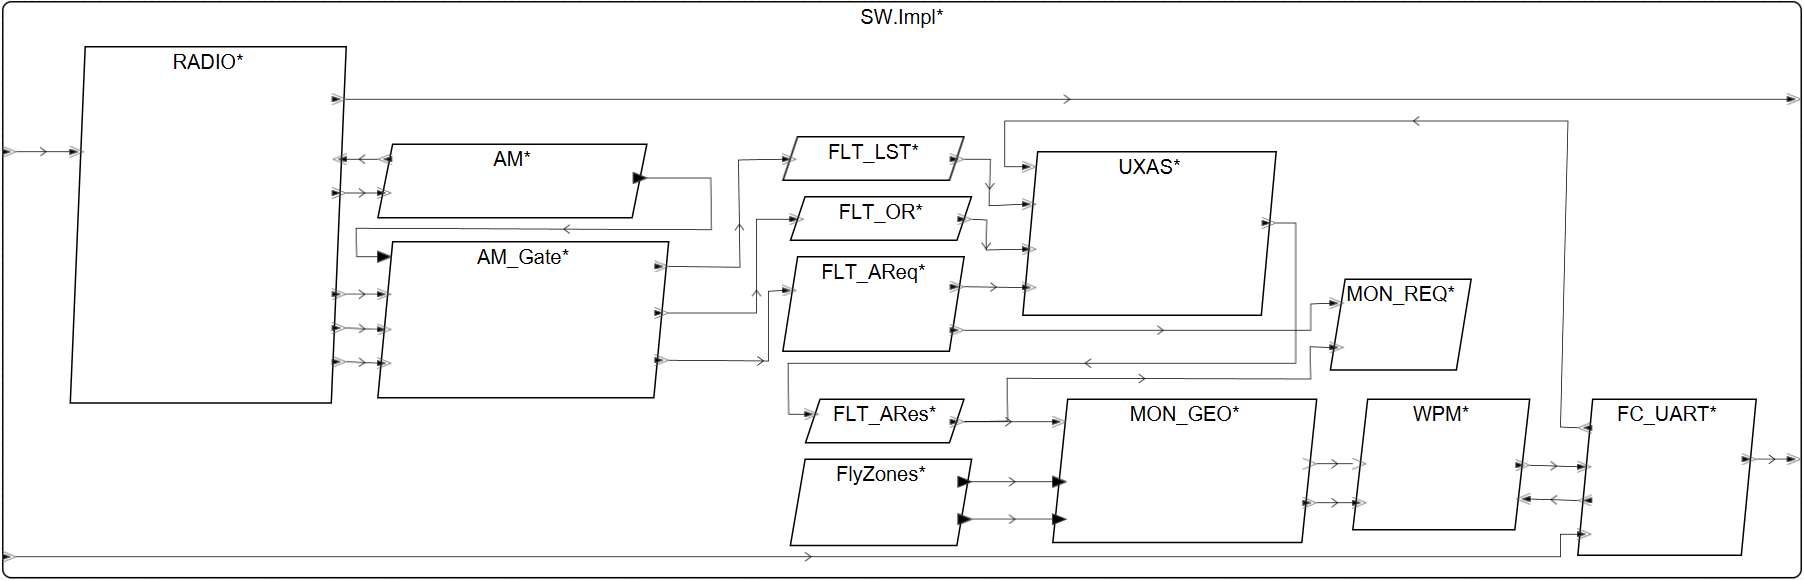
\includegraphics[width=120mm]{sw4.png}
\caption{UAV Software Architecture Model in AADL \label{SW}}
\end{figure}

The hardened model (baseline plus high-assurance components) contained 13 threads,
all of which were mapped to a single mission computer processor running the seL4 microkernel (chosen for its formally verified separation guarantees).
An seL4 domain schedule was added to the model with all threads designated to run once per scheduling cycle with a period of 500 ms.
The processor time allocated to each thread ranged from 2 ms (filters and monitors) to 100 ms (UxAS).
The verification goal was to prove that the key system security properties were satisfied by the hardened model with the components executing according to the seL4 domain schedule.

We note that although \textit{event} and \textit{event data} ports were used in the UAV AADL model, they were intended to model the event-triggered execution of periodic threads.
In addition, since each thread executed once every scheduling cycle, the number of queued events or data was always equal to or less than one,
making this model suitable for the application of our modeling framework.

The following system-level security properties were to be verified in the presence of the seL4 domain schedule:
(a) the output UART and RF messages are \emph{well-formed},
(b) the system only responds to trusted sources, and
(c) the waypoints generated are \emph{geo-fenced}.
% \begin{itemize}
% 	\item The output UART and RF messages are \emph{well-formed}
% 	\item The system only responds to trusted sources
% 	\item The waypoints generated are \emph{geo-fenced}
% \end{itemize}
The encoding of the well-formedness property and its assumptions is shown in Figure~\ref{wellformed}. 

\begin{figure}[t!]
\centering
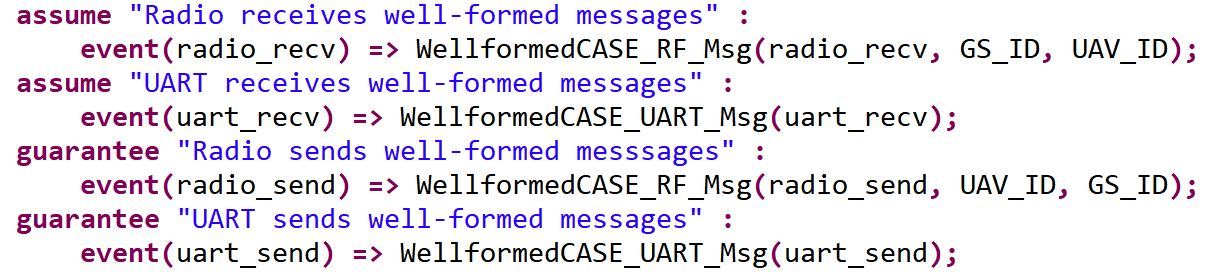
\includegraphics[width=90mm]{wellformed.jpg}
\caption{Assumptions and Well-formedness Properties Modeled in AGREE \label{wellformed}}
\end{figure}

\begin{figure}[t!]
\centering
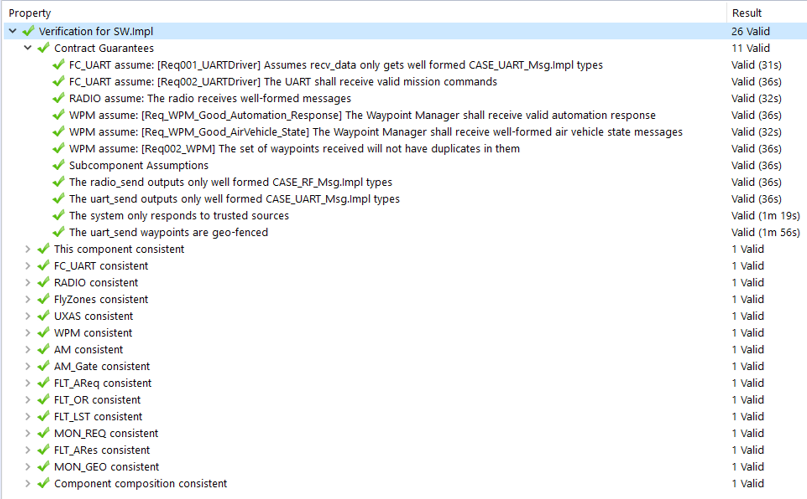
\includegraphics[width=110mm]{proof.png}
\caption{Use Case Verification Results in AGREE \label{proof}}
\end{figure}

Our framework was able to prove these properties in less than 2 minutes on a PC with 2.6 GHz CPU and 32 GB RAM. The verification results is shown in Figure~\ref{proof}. 

The case study is reflective of a development workflow in which we first verify that the component contracts hold under a synchronous dataflow model.  As the design is refined and an execution schedule for each component is specified, we want to show that the system properties continue to hold.  Our new framework enables such verification, providing assurance of intended behavior at runtime. 